\section{Front and Rear Distance}
\label{sec:02_distance}

For simplicity, the direction of the sound source is determined in
horizontal plane only.
However, the front and rear microphones differ 0.0212\si{m} in height
what can provide rough information about the distance of the sound source
for the particular case when the signal comes straight from front or behind.
If $delay_{01}$ and $delay_{32}$ are both very small, the signal comes from
the front or the back most likely.
Figure ...\missing[]{reference to nao channel figure} evinces, that one of
the sidewise delays need to be larger or equal to 5.41 \change[]{number to variable?}
samples for a signal to arrive from sideways.
When the delays of the side channels are smaller, they can be used to
detect the angle of the sound source in vertical YZ plane.

Figure \cref{fig:02_headSideTdoa} is a lateral illustration of
the Nao's right microphones $channel_1$ and $channel_3$.
% -------------------------------------------------------------
\begin{figure}[ht]
	\centering
		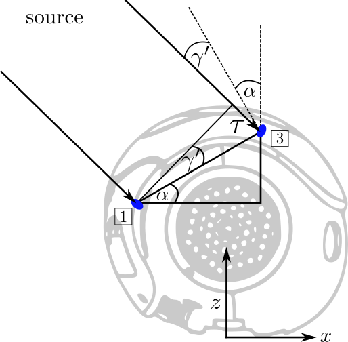
\includegraphics[width=0.45\columnwidth]{figures/side_head_tdoa}
	\caption{}
    \label{fig:02_headSideTdoa}
\end{figure}
% -------------------------------------------------------------
With the delay samples $\tau$, the angle of the sound source $\gamma$ relative
to the Z-axis can be determined with
% -------------------------------------------------------------
\bsub \bal
\gamma &= \alpha + \gamma'\\
\gamma' &= sign(delay) \cdot sin^{-1}(\frac{delay}{samples_{max}})\\
\intertext{with}
\alpha &= tan^{-1}(\frac{\Delta z_{channel}}{\Delta x_{channel}})
\eal \esub
which is the angle to the orthogonal axis to the plane though
front and rear channels.
% -------------------------------------------------------------
\begin{figure}[ht]
	\centering
		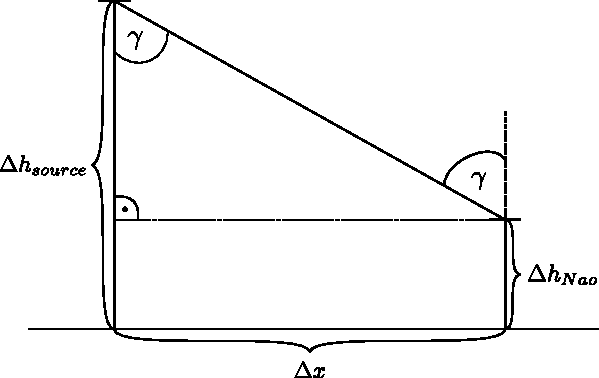
\includegraphics[width=0.6\columnwidth]{figures/x_distance}
	\caption{}
    \label{fig:02_xDistance}
\end{figure}
% -------------------------------------------------------------
Known that the sound source is positioned above of the robot, the distance
of the sound source can be approximated with an assumed height $\Delta h_{source}$
of the source.
So, the distance to the sound source is
% -------------------------------------------------------------
\bal
\Delta x &= (\Delta h_{source} - \Delta h_{Nao}) \cdot \tan(\gamma).
\label{eq:02_deltaX}
\eal
% -------------------------------------------------------------